%%%%%%%%%%%%%%%%%%%%%%%%%%%%%%%%%%%%%%%%%%%%%%%%%%%%%%%%%%%%%%%%%%%%%%%%%%%%%%%%
%2345678901234567890123456789012345678901234567890123456789012345678901234567890
%        1         2         3         4         5         6         7         8

\documentclass[letterpaper, 10 pt, conference]{ieeeconf}  % Comment this line out
                                                          % if you need a4paper
%\documentclass[a4paper, 10pt, conference]{ieeeconf}      % Use this line for a4
                                                          % paper

\IEEEoverridecommandlockouts   
\usepackage{booktabs}
% This command is only
                                                          % needed if you want to
                                                          % use the \thanks command
\overrideIEEEmargins
% See the \addtolength command later in the file to balance the column lengths
% on the last page of the document



% The following packages can be found on http:\\www.ctan.org
\usepackage{graphicx} % for pdf, bitmapped graphics files
%\usepackage{epsfig} % for postscript graphics files
%\usepackage{mathptmx} % assumes new font selection scheme installed
%\usepackage{times} % assumes new font selection scheme installed
%\usepackage{amsmath} % assumes amsmath package installed
%\usepackage{amssymb}  % assumes amsmath package installed
\usepackage{cite} % takes care of citations

\title{\LARGE \bf
"The smell of fear" - In Search of Patterns Between Emotions and Breath Composition - Data Cleaning
}


\author{Jason Tam$^{1}$\thanks{{\tt\small $^{1}$jtam013@aucklanduni.ac.nz}}, Musa Abdel-Rahman$^{2}$\thanks{{\tt\small $^{2}$mabd292@aucklanduni.ac.nz}}, Catherine Liu$^{3}$\thanks{{\tt\small $^{3}$cliu129@aucklanduni.ac.nz}}\\Supervised by J{\"o}rg Wicker}

\begin{document}

\maketitle
\thispagestyle{empty}
\pagestyle{empty}

%%%%%%%%%%%%%%%%%%%%%%%%%%%%%%%%%%%%%%%%%%%%%%%%%%%%%%%%%%%%%%%%%%%%%%%%%%%%%%%%

%\begin{abstract}

%This is where the abstract goes, if we decide to have one

%\end{abstract}

%%%%%%%%%%%%%%%%%%%%%%%%%%%%%%%%%%%%%%%%%%%%%%%%%%%%%%%%%%%%%%%%%%%%%%%%%%%%%%%%

\section{ALIGNMENT AND EXCLUSION OF SESSIONS}

As the objective of this study is to determine if potential associations are present between the scene labels and the gas content detected in theatre, data collected from different sessions are grouped by the movie played for analysis.

With the relationship between CO$_2$ and human breath composition being the best understood compared to other available gas channels of the detector, data from the CO$_2$ channel is used to determine the general effect from the audience. Figure \ref{BuddyUncleaned} shows the data from the CO$_2$ channel collected from all sessions of the movie 'Buddy'. It is clear that while the traces for most of the sessions followed a general pattern, a small number of them has distinctive difference in shape. Some of the differences are emphasized in the normalized data shown in Figure \ref{BuddyUncleanedNormed}.

\begin{figure}[thpb]
  \centering
  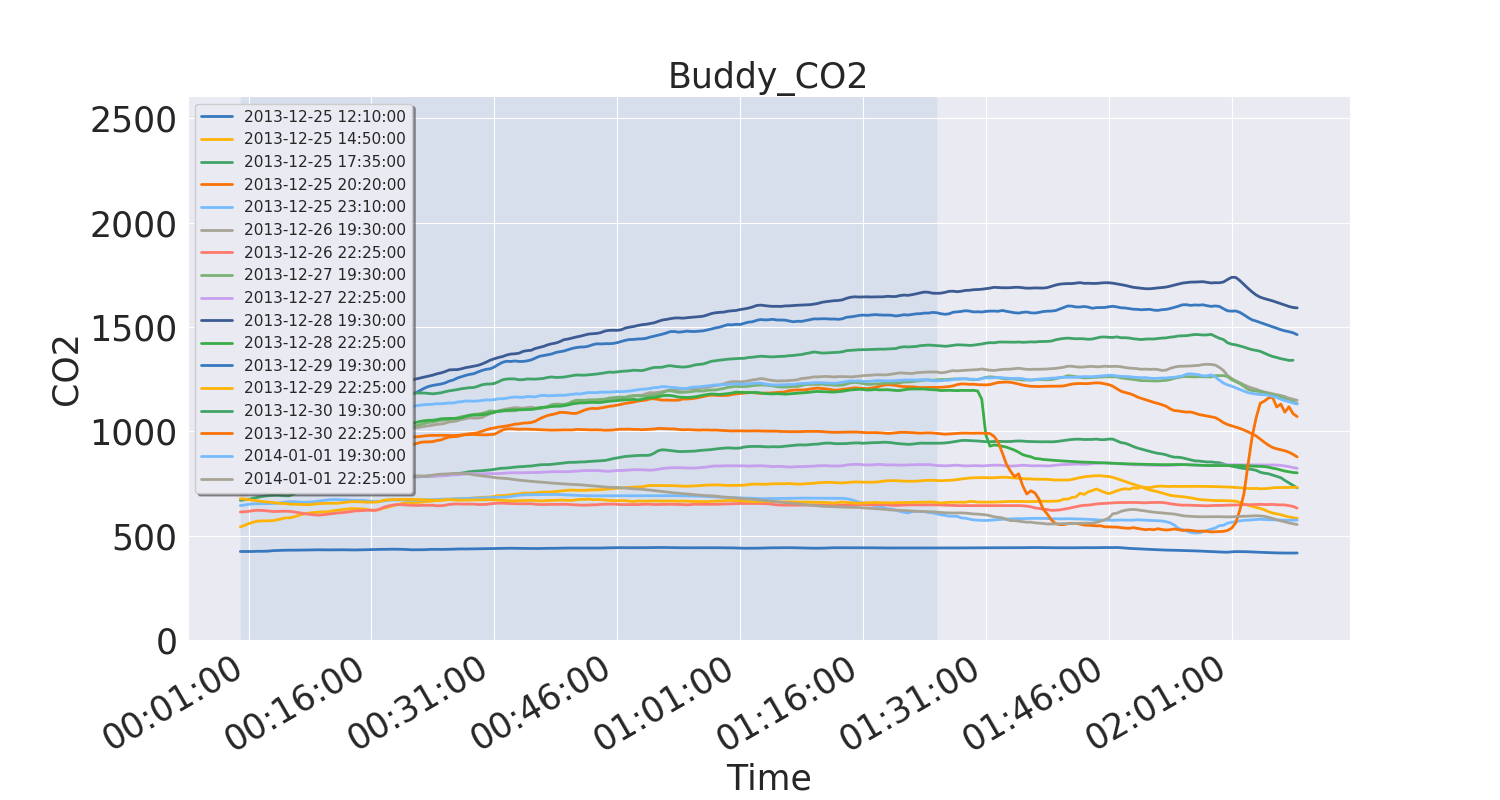
\includegraphics[width=0.47\textwidth]{../Plots/uncleanedCO2/Buddy_CO2.png}
  \caption{Uncleaned sessions data of 'Buddy'}
  \label{BuddyUncleaned}
\end{figure}

\begin{figure}[thpb]
  \centering
  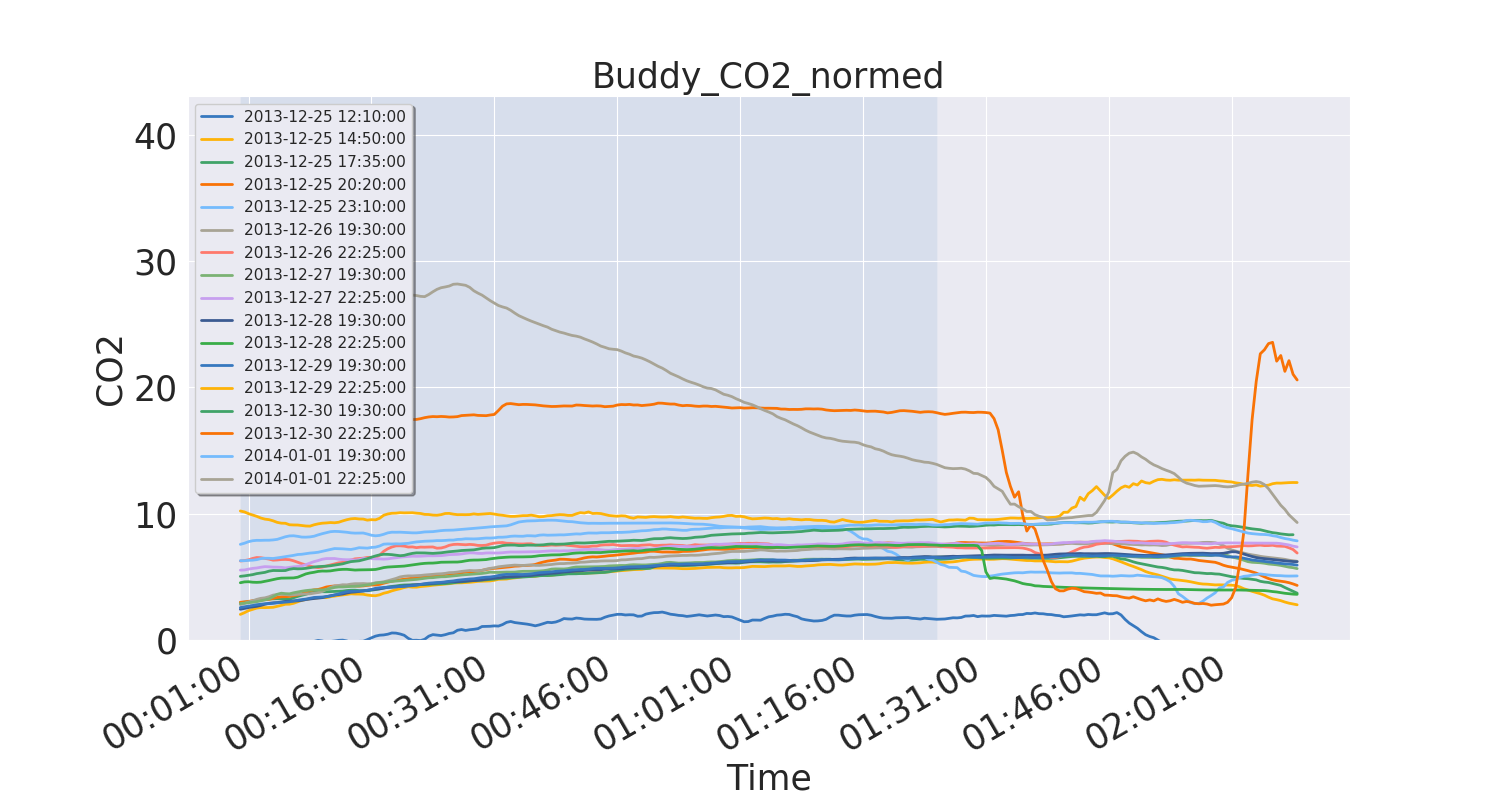
\includegraphics[width=0.47\textwidth]{../Plots/uncleanedCO2/Buddy_CO2_normed.png}
  \caption{Uncleaned and normalized sessions data of 'Buddy'}
  \label{BuddyUncleanedNormed}
\end{figure}

The starting time for all of these sessions plotted in the graph are aligned with the 'begin' time provided in the data. The shaded area represent the duration of the movie using the aligned starting time, with the ending time estimated by the number of columns that represent 30 second intervals in the scene label data table. Data of extended time periods (45 minutes) after the estimated ending time are included to more accurately determine the ending time of the movie, as it can be safely assumed that delays that affect the true starting time of the movie are not uncommon. It is also assume that a noticable drop in CO$_2$ counts would occur as the audience leave the theatre after the end of the movie, and this is used to align the playing time of the movie across different sessions. The aligned data for the 'Buddy' movie is shown in Figures \ref{BuddyCleaned} and \ref{BuddyCleanedNormed}.

\begin{figure}[thpb]
  \centering
  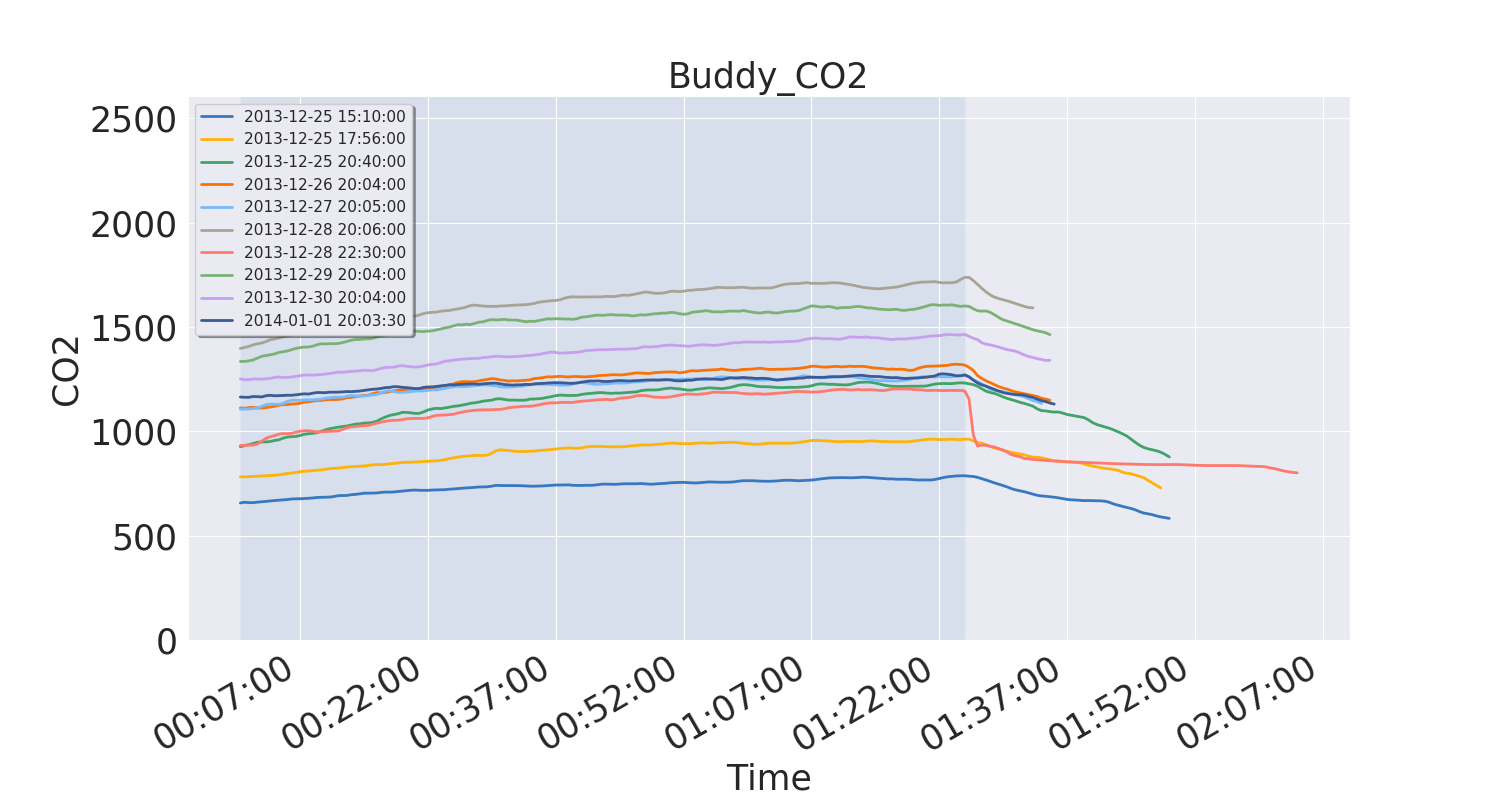
\includegraphics[width=0.47\textwidth]{../Plots/Buddy_CO2.png}
  \caption{Cleaned sessions data of 'Buddy'}
  \label{BuddyCleaned}
\end{figure}

\begin{figure}[thpb]
  \centering
  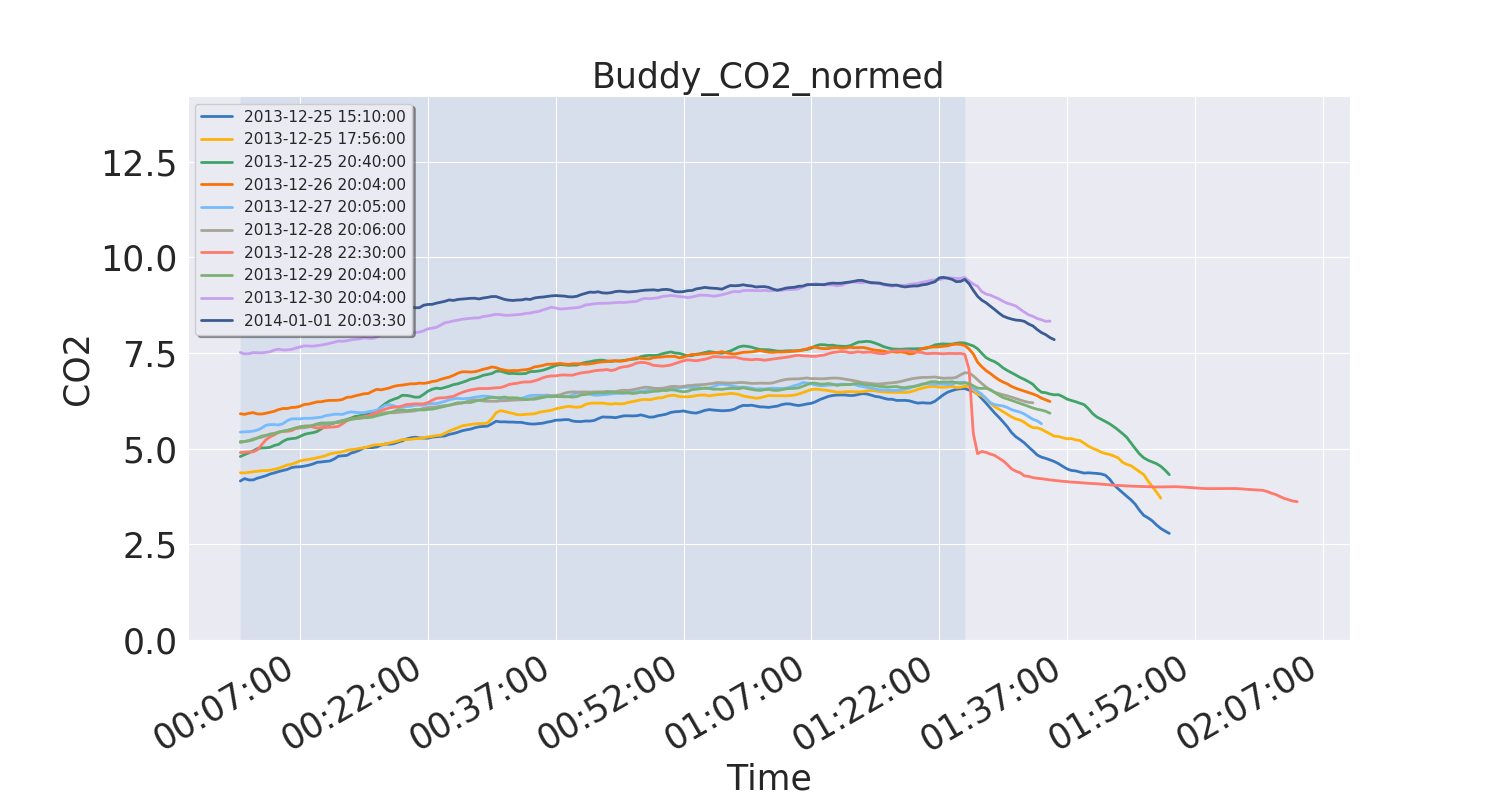
\includegraphics[width=0.47\textwidth]{../Plots/Buddy_CO2_normed.png}
  \caption{Cleaned and normalized sessions data of 'Buddy'}
  \label{BuddyCleanedNormed}
\end{figure} 

This data cleaning strategy seems to be appropriate as there are still a good number of remaining sessions for further analysis. Similar results were obtained for 'The Hunger Games: Cathcing Fire' and 'Walter Mitty', as shown respectively in Figures \ref{TributeCleanedNormed} and \ref{WalterMittyCleanedNormed}.

\begin{figure}[thpb]
  \centering
  \includegraphics[width=0.47\textwidth]{"../Plots/The Hunger Games: Catching Fire_CO2_normed".png}
  \caption{Cleaned sessions data of 'The Hunger Games: Ctaching Fire'}
  \label{TributeCleanedNormed}
\end{figure}

\begin{figure}[thpb]
  \centering
  \includegraphics[width=0.47\textwidth]{"../Plots/Walter Mitty_CO2_normed".png}
  \caption{Cleaned and normalized sessions data of 'Walter Mitty'}
  \label{WalterMittyCleanedNormed}
\end{figure}

However the same cannot be said with the other movies. 'Machete Kills' only has two sessions, and only one of the two sessions can be aligned with the same logic, as the CO$_2$ count in the other trace starts to noticably drop before reaching the length of the movie. The two sessions are shown in Figure \ref{MacheteKillsCleanedNormed}, and whether the aligned session has enough value to keep for the analysis is open for discussion.

\begin{figure}[thpb]
  \centering
  \includegraphics[width=0.47\textwidth]{"../Plots/Machete Kills_CO2_normed".png}
  \caption{Cleaned and normalized sessions data of 'Machete Kills'}
  \label{MacheteKillsCleanedNormed}
\end{figure}

Even with 45 minutes of extended time considered, noticable drop in counts for the CO$_2$ channel does not appear in any sessions of 'Hobbit 2' and 'Paranormal Activity'. These are shown in Figure \ref{HobbitUncleaned} - \ref{ParanormalActivityUncleanedNormed}.

\begin{figure}[thpb]
  \centering
  \includegraphics[width=0.47\textwidth]{"../Plots/uncleanedCO2/Hobbit 2_CO2".png}
  \caption{Uncleaned sessions data of 'Hobbit 2'}
  \label{HobbitUncleaned}
\end{figure}

\begin{figure}[thpb]
  \centering
  \includegraphics[width=0.47\textwidth]{"../Plots/uncleanedCO2/Hobbit 2_CO2_normed".png}
  \caption{Uncleaned and normalized sessions data of 'Hobbit 2'}
  \label{HobbitUncleanedNormed}
\end{figure}

\begin{figure}[thpb]
  \centering
  \includegraphics[width=0.47\textwidth]{"../Plots/uncleanedCO2/Paranormal Activity_CO2".png}
  \caption{Uncleaned sessions data of 'Paranormal Activity'}
  \label{ParanormalActivityUncleaned}
\end{figure}

\begin{figure}[thpb]
  \centering
  \includegraphics[width=0.47\textwidth]{"../Plots/uncleanedCO2/Paranormal Activity_CO2_normed".png}
  \caption{Uncleaned and normalized sessions data of 'Paranormal Activity'}
  \label{ParanormalActivityUncleanedNormed}
\end{figure}

Particularly for 'Paranormal Activity', there seem to be two main types of patterns for different sessions, possibly due to the aftermath of the sessions before. Whether the sessions of these two movies have enough value to keep for the analysis is also open for discussion, while I can look further into the extended time periods to look for a similar drop in counts to hopefully perform the same alignment. I have excluded all three of these movies ['Machete Kills', 'Hobbit 2', 'Paranormal Activity'] for now and produced an updated CSV file for clustering analysis. The dataset contained within should be the cleanest subset available, whether the quantity is adequate for the analysis can be examined from the results obtained, and the strategy can be further refined if needed.

\addtolength{\textheight}{-12cm}   % This command serves to balance the column lengths
                                  % on the last page of the document manually. It shortens
                                  % the textheight of the last page by a suitable amount.
                                  % This command does not take effect until the next page
                                  % so it should come on the page before the last. Make
                                  % sure that you do not shorten the textheight too much.

%%%%%%%%%%%%%%%%%%%%%%%%%%%%%%%%%%%%%%%%%%%%%%%%%%%%%%%%%%%%%%%%%%%%%%%%%%%%%%%%



%%%%%%%%%%%%%%%%%%%%%%%%%%%%%%%%%%%%%%%%%%%%%%%%%%%%%%%%%%%%%%%%%%%%%%%%%%%%%%%%



%%%%%%%%%%%%%%%%%%%%%%%%%%%%%%%%%%%%%%%%%%%%%%%%%%%%%%%%%%%%%%%%%%%%%%%%%%%%%%%%
%\section*{APPENDIX}

%Appendixes should appear before the acknowledgment.

%\section*{ACKNOWLEDGMENT}

%The preferred spelling of the word ÒacknowledgmentÓ in America is without an ÒeÓ after the ÒgÓ. Avoid the stilted expression, ÒOne of us (R. B. G.) thanks . . .Ó  Instead, try ÒR. B. G. thanksÓ. Put sponsor acknowledgments in the unnumbered footnote on the first page.



%%%%%%%%%%%%%%%%%%%%%%%%%%%%%%%%%%%%%%%%%%%%%%%%%%%%%%%%%%%%%%%%%%%%%%%%%%%%%%%%

%References are important to the reader; therefore, each citation must be complete and correct. If at all possible, references should be commonly available publications.


% \bibliographystyle{ieeetr}
% \bibliography{LitSurvey.bib}


\end{document}
